This master thesis has been carried out at Khademhosseini laboratory, Harvard-MIT Health Science and Technology (Brigham and Women's Hospital), in Cambridge, MA.\\
During my six-months of research I have joined \textit{\textbf{XCEL}} grant project, a five years project sponsored by the U.S. Defense Threat Reduction Agency (\textit{DTRA}).

The goal of this project is to develop a system, a microscale bioreactor containg four 3D fully-functional \textit{organs-on-a-chip}.

\begin{figure}[h]
	\centering
	\includegraphics[width = 0.8\textwidth]{Intro/body}
	\caption{\textit{XCEL} project (\textit{Body-on-a-chip})}
	\label{Fig:Body}
	
\end{figure}

The (Fig.\ref{Fig:Body}) shows, in a schematic representation, the design of the entire \textit{XCEL} project. On the breadboard four organs are connected from each others: liver, heart, ling, and vascular system (\textit{Vasc}). The medium used to connect them is using tubing circuit where the media flows. This tubing connections are driven by electrovalves.


My role in this project has been to create a custom user interface on Google Glass for simultaneous recording of biosensing data such as temperature, pH, and microscopy images/videos as well as remote control of the microfluidic valves previously introduced. In summary my aim was to design a Google Glass App for use in organs-on-a-chip platforms.

The \textit{organs-on-a-chip} platforms contain interconnected microfluidic modular components including the bioreactors for hosting biomimicry human organ models, downstream biochemical sensors to continually monitor the levels of biomarkers secreted by the organs, and physical sensors to monitor the physical microenvironment of the circulatory system. Due to their extensive similarity with human organs, these miniature human models are finding widespread applications where the prediction of in vivo responses of the human body is needed, including but not limited to drug screening, basic biomedical studies, and environmental safety assessment. Thus, the \textit{organs-on-a-chip} platforms seek to recapitulate human organ function at micro-scale by integrating microfluidic networks with three-dimensional organ models, which are expected to provide robust and accurate predictions of drug/toxin effects in human bodies. In fulfilling this aim, a set of physical/chemical parameters need to be monitored and stored in order to capture such effects of drug/toxin administered into the system.\\

By precisely designing the Google Glass App for this organs-on-a-chip platform it allows convenient observation and control of the organ models, biosensors, and the microfluidic circuitry, which has been difficult to achieve previously.

The system designed and described in this thesis is illustrated in (Fig.\ref{Fig:BlockDiagram}).
 
 \begin{figure}[h]
 	\centering
 	\includegraphics[width = \textwidth]{Intro/Block_Diagram.eps}
 	\caption{Block diagram of the system}
 	\label{Fig:BlockDiagram}
 	
 \end{figure}
 
 The (Fig.\ref{Fig:BlockDiagram}) shows the principal steps of data transmission from physical and video sensors to the Google Glass via an \textit{Embedded Linux System} performed using the \href{http://beagleboard.org/BLACK}{\textbf{Beaglebone Black}}.\\
 The Beaglebone Black runs processes that are in charged to:
 \begin{itemize}
 	\item acquire the sensors value and to store them onto \textit{Google App Engine Data Storage};
 	\item acquire the video, perform the beating plot, and to store them onto \textit{Google App Engine Data Storage};
 	\item get from the \textit{Google App Engine Data Storage} the electrovalves status set from the user through the Google Glass and to drive the electrovalves.
 \end{itemize} 
 
 The whole designed environment includes a program, written using the framework \textit{Qt}, for storing the recorded video from microscope.
 
 \section*{The Glasswear}
 \addcontentsline{toc}{section}{The Glasswear}
 The (Fig.\ref{Fig:GlasswearDiagram}) shows the structure of the Glasswear. From the Home Screen (Fig.\ref{Fig:GlasswearDiagram}a), using the voice trigger "\textit{Show Measurement}" or tapping on the "\textit{Measurement}" card (Fig.\ref{Fig:GlasswearDiagram}b) user is allowed to enter in the application (Fig.\ref{Fig:GlasswearDiagram}c). From this point, tapping and swiping, it's possible to navigate into the glasswear's menu (Fig.\ref{Fig:GlasswearDiagram}d-h) and choose which card has to be shown. \textit{View PH} (Fig.\ref{Fig:GlasswearDiagram}i) and \textit{View Temperature} (Fig.\ref{Fig:GlasswearDiagram}j) cards  plot on the card's left side the value of pH and temperature, respectively. While on the right side they show the average value. The microscope's video is shown by tapping on \textit{View Video} (Fig.\ref{Fig:GlasswearDiagram}k). The \textit{View Beating} card shows the graph of the beating associated to the video.
 \\
 
 \begin{figure}[h]
 	\centering
	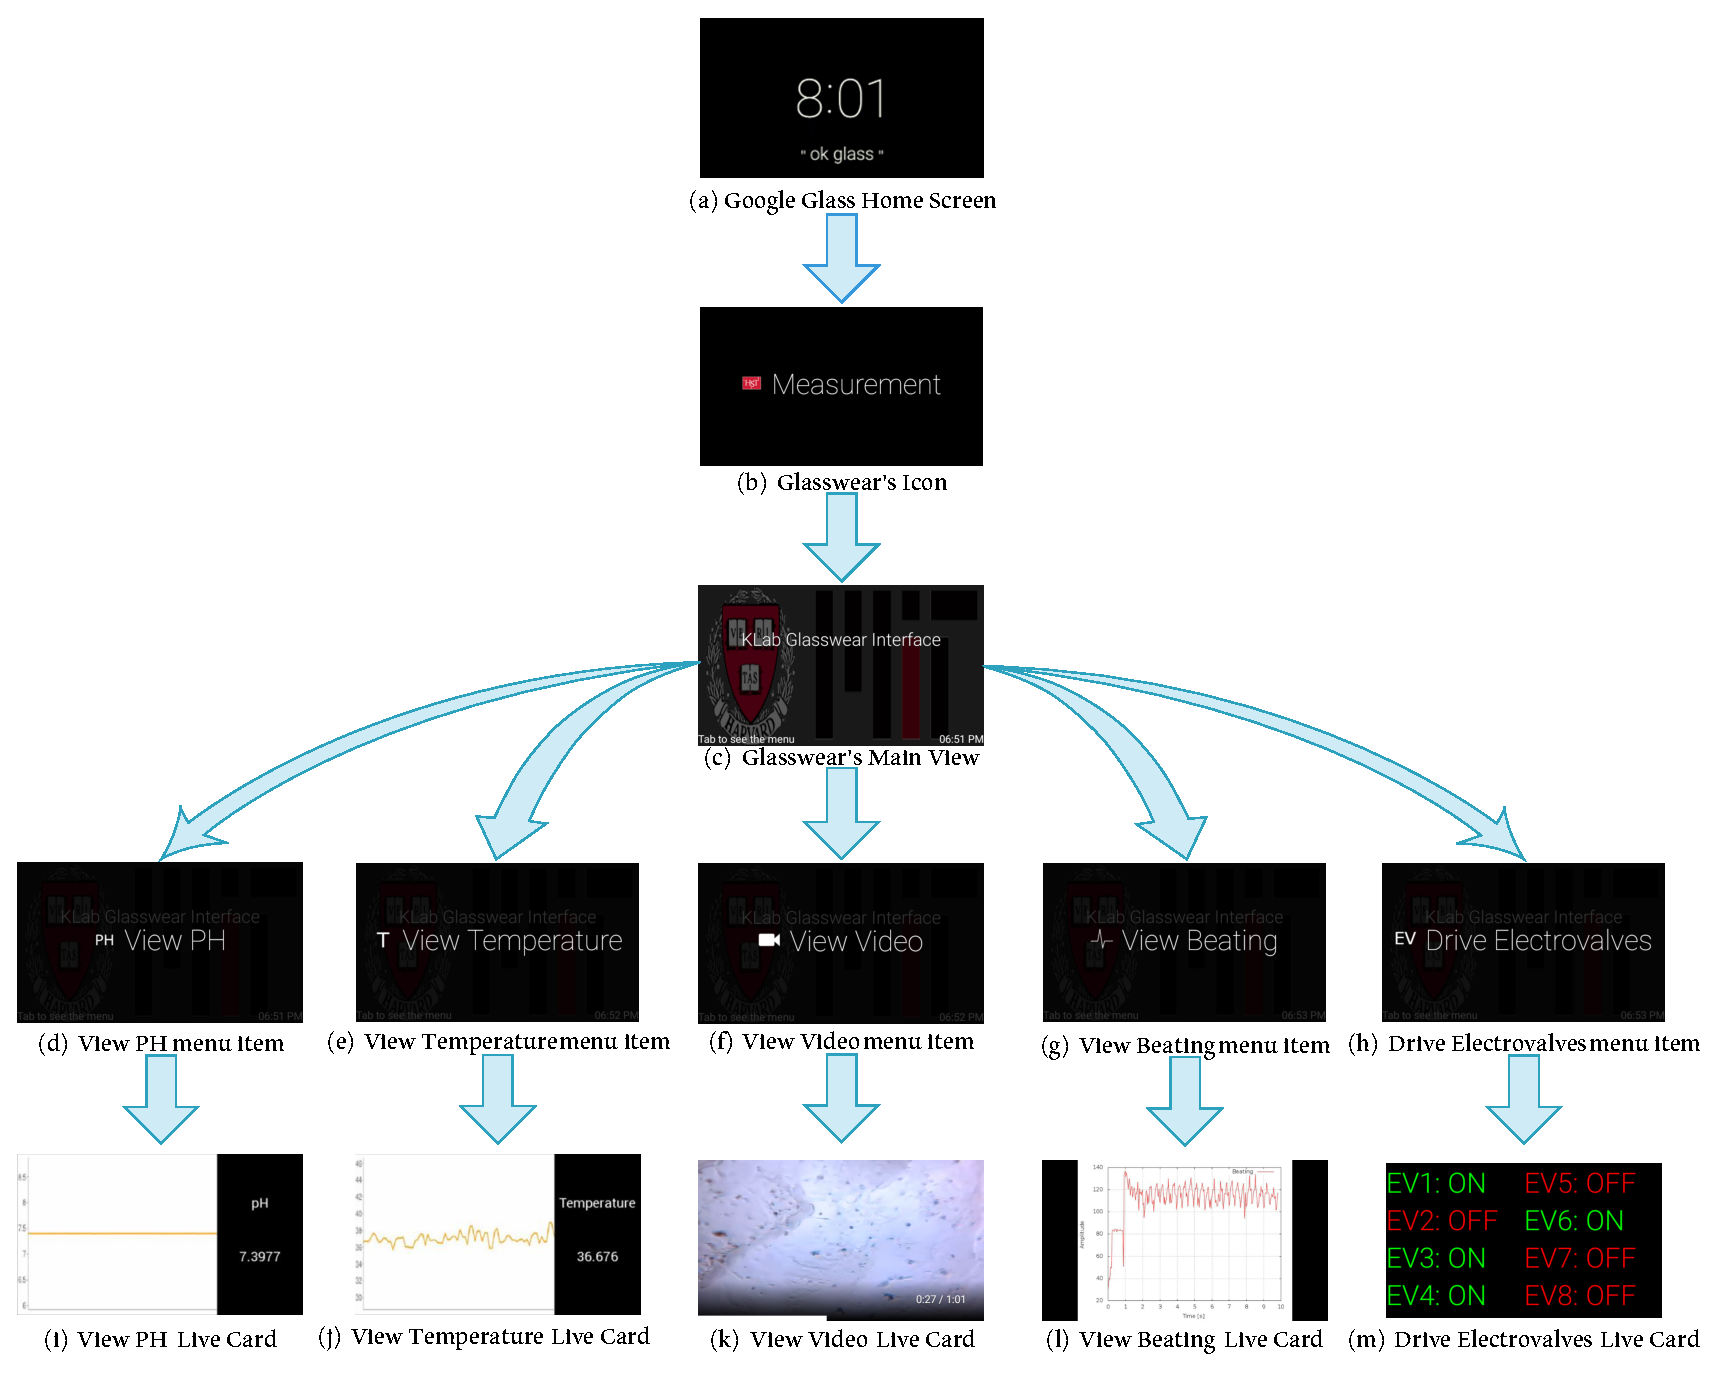
\includegraphics[width=\textwidth]{Intro/block-app.eps}
 	\caption{Glasswear's Block Diagram}
 	\label{Fig:GlasswearDiagram}
 \end{figure}

 
 From the \textit{Drive Electrovalves} card (Fig.\ref{Fig:GlasswearDiagram}m), the user can set the value of each electrovalve. The main view of this card shows the status of each electrovalve (written in green if it is on and in red if it is off).
 \clearpage
 \begin{figure}[h]
 	\centering
 	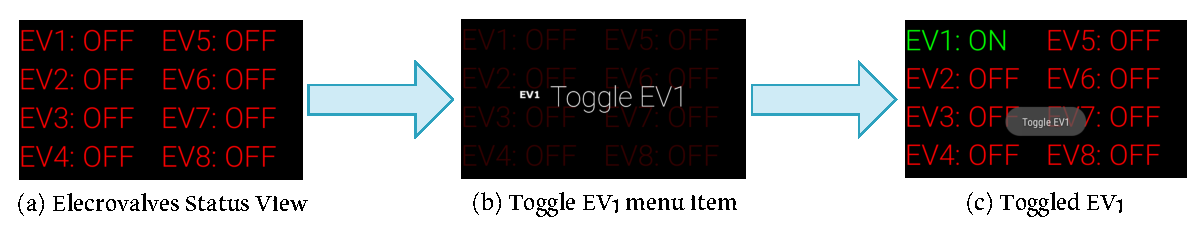
\includegraphics[width=\textwidth]{Intro/electrovalves.eps}
 	\caption{Drive Electrovalves Steps}
 	\label{Fig:Electrovalves}
 \end{figure}
 
 The (Fig.\ref{Fig:Electrovalves}) shows the steps to toggle the status of the first electrovalve:
 \begin{enumerate}
 	\item (Fig.\ref{Fig:Electrovalves}a) shows the initial status of the whole electrovalves (all off);
 	\item tapping on the card and swiping the user is allowed to change the status of each electrovalve from the menu, as shown in (Fig.\ref{Fig:Electrovalves}b);
 	\item after that the electrovalve has been chosen, a toast message pops up (Fig.\ref{Fig:Electrovalves}c), and the new values of the electrovalves are shown. 
 \end{enumerate}
 
 To return on the main card of the glassware, the user has to tab on \textit{Back} item (Fig.\ref{Fig:Back}) from every menu.
 
 \begin{figure}[h]
 	\centering
 	\includegraphics[scale=.35]{Intro/back_menu}
 	\caption{\textit{Back} menu item}
 	\label{Fig:Back}
 \end{figure}
 
 To terminate the glassware, from every menu, the user has to swipe up to the final item and tab on \textit{Exit} item (Fig.\ref{Fig:Exit}).
 
 \begin{figure}[h]
 	\centering
 	\includegraphics[scale=.35]{Intro/exit}
 	\caption{\textit{Exit} menu item}
 	\label{Fig:Exit}
 \end{figure}
 
\section*{The Board}
\addcontentsline{toc}{section}{The Board}
\begin{figure}[h]
	\begin{center}
		\includegraphics[width=\textwidth]{thboard}
		\caption{The Board}
		\label{Fig:board}
	\end{center}
\end{figure}

The (Fig.\ref{Fig:board}) shows the top view of the system board. As can be seen it is composed by different interface and connections:
\begin{itemize}
	\item $5\ V$ power supply, required by the microcomputer on the Baglebone Black and by the conditiong circuits on the \textit{PCB};
	\item $24\ V$ power supply, required by the electrovalves;
	\item \textit{Ethernet}, to connect the board to the Internet;
	\item \textit{USB} connection, for the microscope;
	\item \textit{pH header}, to connect the pH sensor\footnote{\textbf{WARNING}: to ensure the correct functionality, user has to pay attention at this connection, since the pH sensor is a passive one, it has a polarity. The positive pin of the sensor has to be connected to the right terminal, looking fro the top (as shown in (Fig.\ref{Fig:board}))};
	\item \textit{temperature header}, to connect the temperature sensor;
	\item \textit{electrovalves header}, made by eight pairs of terminals, ordered as shown in (Fig.\ref{Fig:board}), from the top to the bottom.
\end{itemize}

The remaining two headers, shown in the top left corner of (Fig.\ref{Fig:board}) are thought for future application. In particular they are going to be useful for all those jobs that don't required the interaction with Google Glass, such as sensors calibration.

\section*{Video Storing}
\addcontentsline{toc}{section}{Video Storing}
The storing of the microscope video plays an important role of this system. It may be essential to review the recorded video  during the experiment and in order to fulfill this aim a \textit{Qt} program has been designed.\\
We chose \textit{Qt} because in this way the program is available for different operating systems, \textit{Linux}, \textit{Windows}, and \textit{MacOS}.\\

The program is very easy to use, the user just has to run the executable (Fig.\ref{Fig:icostoring}).

\begin{figure}[h]
	\begin{center}
		\includegraphics[scale=.5]{storing/Icon}
		\caption{Storing Microscope Video Program's Icon}
		\label{Fig:icostoring}
	\end{center}
\end{figure}

Once it has been launched, a console is opened (Fig.\ref{Fig:storingwindows}). The program checks every 20 seconds if a new video has been uploaded on the server. If so, the new video will be stored inside the computer (directory \texttt{C:/Video}) with the current data and hour as name in the following form: $YYYY-MM-DD-HH-mmss$, as shown in (Fig.\ref{Fig:stored}).\\

As shown in (Fig.\ref{Fig:storingwindows}) on the console the user can read all the information about what the program is doing.

\begin{figure}[h]
	\begin{center}
		\includegraphics[width=\textwidth]{storing/program-windows}
		\caption{Storing Microscope Video Console}
		\label{Fig:storingwindows}
	\end{center}
\end{figure}

\begin{figure}[h]
	\begin{center}
		\includegraphics[width=\textwidth]{storing/stored}
		\caption{Video Stored in the Folder}
		\label{Fig:stored}
	\end{center}
\end{figure}
 
 
